%!TEX root = ../dissertation.tex
%\begin{savequote}[75mm]
%Nulla facilisi. In vel sem. Morbi id urna in diam %dignissim feugiat. Proin molestie tortor eu velit. %Aliquam erat volutpat. Nullam ultrices, diam tempus %vulputate egestas, eros pede varius leo.
%\qauthor{Quoteauthor Lastname}
%\end{savequote}

\chapter{Algoritmos implementados}

%\newthought{There's something to be said}
En este capítulo se revisan los seis algoritmos de preprocesamiento y clasificación de datos ordinales y monotónicos implementados en el paquete software desarrollado, ofreciendo una descripción teórica de los mismos. Para ello se divide el capítutlo en dos secciones: algoritmos de preprocesamiento y algoritmos de clasificación.
\section{Preprocesamiento}
\subsection{Selector de características para clasificación monotónica}
Se implementa en el paquete el algoritmo para selección de características \cite{hu2012feature} basado en Rank Mutual Information. El funcionamiento del algoritmo propuesto por Qinghua Hu et Al. es el siguiente: \newline
 Consideremos un conjunto de datos $\langle U, A, D \rangle$ donde $U$ denota las instancias, $A$ denota los atributos y $D$ las clases, tal que $D=d_1 < d_2 < ... < d_k$. Entonces, para cada atributo $a \in A$ se calculan las relaciones entre las instancias usando la siguiente función \textit{logsig}: 
 $$r_{ij}^{<}=\frac{1}{1+e^{\ k \ ( v(x_i,a)-v(x_j,a) )}}$$
 Donde $v(x_i,a)$ es el valor de la instancia $x_i$ para el atributo $a$, y $k$ es una constante positiva.
 El resultado de aplicar esta función es:
 
\[ 
\left \{
\begin{tabular}{cc}
0.5, & si $r_{ii}^{>}=r_{ii}^{<}$ \\
$\approx 1$, & si $v(x_j,a) >> v(x_i,a)$  \\
$\approx 0$, & si $v(x_j,a) << v(x_i,a)$ 
\end{tabular}
\right \}
\]

Es decir, en el primer caso no habría diferencia entre $x_i$ y $x_j$, en el segundo caso $x_i$ sería significativamente inferior a $x_j$, y en el tercer caso $x_i$ sería significativamente mayor. \newline
Con esto se calculan los conjuntos ordinales difusos mayores que $x_i$ en términos de $a$ de la siguiente forma:
$$[x_i]_a^{\leq}=r_{i1}/x_1 + r_{i2}/x_2 +...+r_{in}/x_n$$
que serán posteriormente usados para calcular la \textit{mutual rank information} entre dos atributos cualesquiera sobre un conjunto de instancias de la siguiente forma: 
$$RMI_{a_1,a_2}(U)= -\sum_{i=1}^{n} \frac{1}{n} \log \frac{| [x_i]_{a_1}^{\leq}| \times |[x_i]_{a_2}^{\leq}|  }{ n \times | [x_i]_{a_1}^{\leq} \cap [x_i]_{a_2}^{\leq} |}$$

Esta ganancia de información se combina junto con la ganancia de información de cada característica con respecto a la clase, obteniendo el criterio mRMR (minimum redundancy maximum relevance), que trata de encontrar las características más significativas y menos relevantes:
$$\Phi=\frac{1}{|B|} \sum_{a_i \in B} RMI_{a_i,D} - \frac{\beta}{|B|^2} \sum_{a_i, a_j \in B} RMI_{a_i,a_j} $$ 
donde $\beta$ es un parámetro regulativo. Finalmente se seleccionan las \textit{$k$} características con mayor mRMR.
\subsection{Selector de instancias para clasificación monotónica}

\section{Clasificación}
\subsection{SVMOP}
%SVMOP Support vector machines using Frank & Hall method for ordinal
% regression (by binary decomposition)
\subsection{POM}
\subsection{KDLOR}
\subsection{WKNN}
%\begin{figure}
%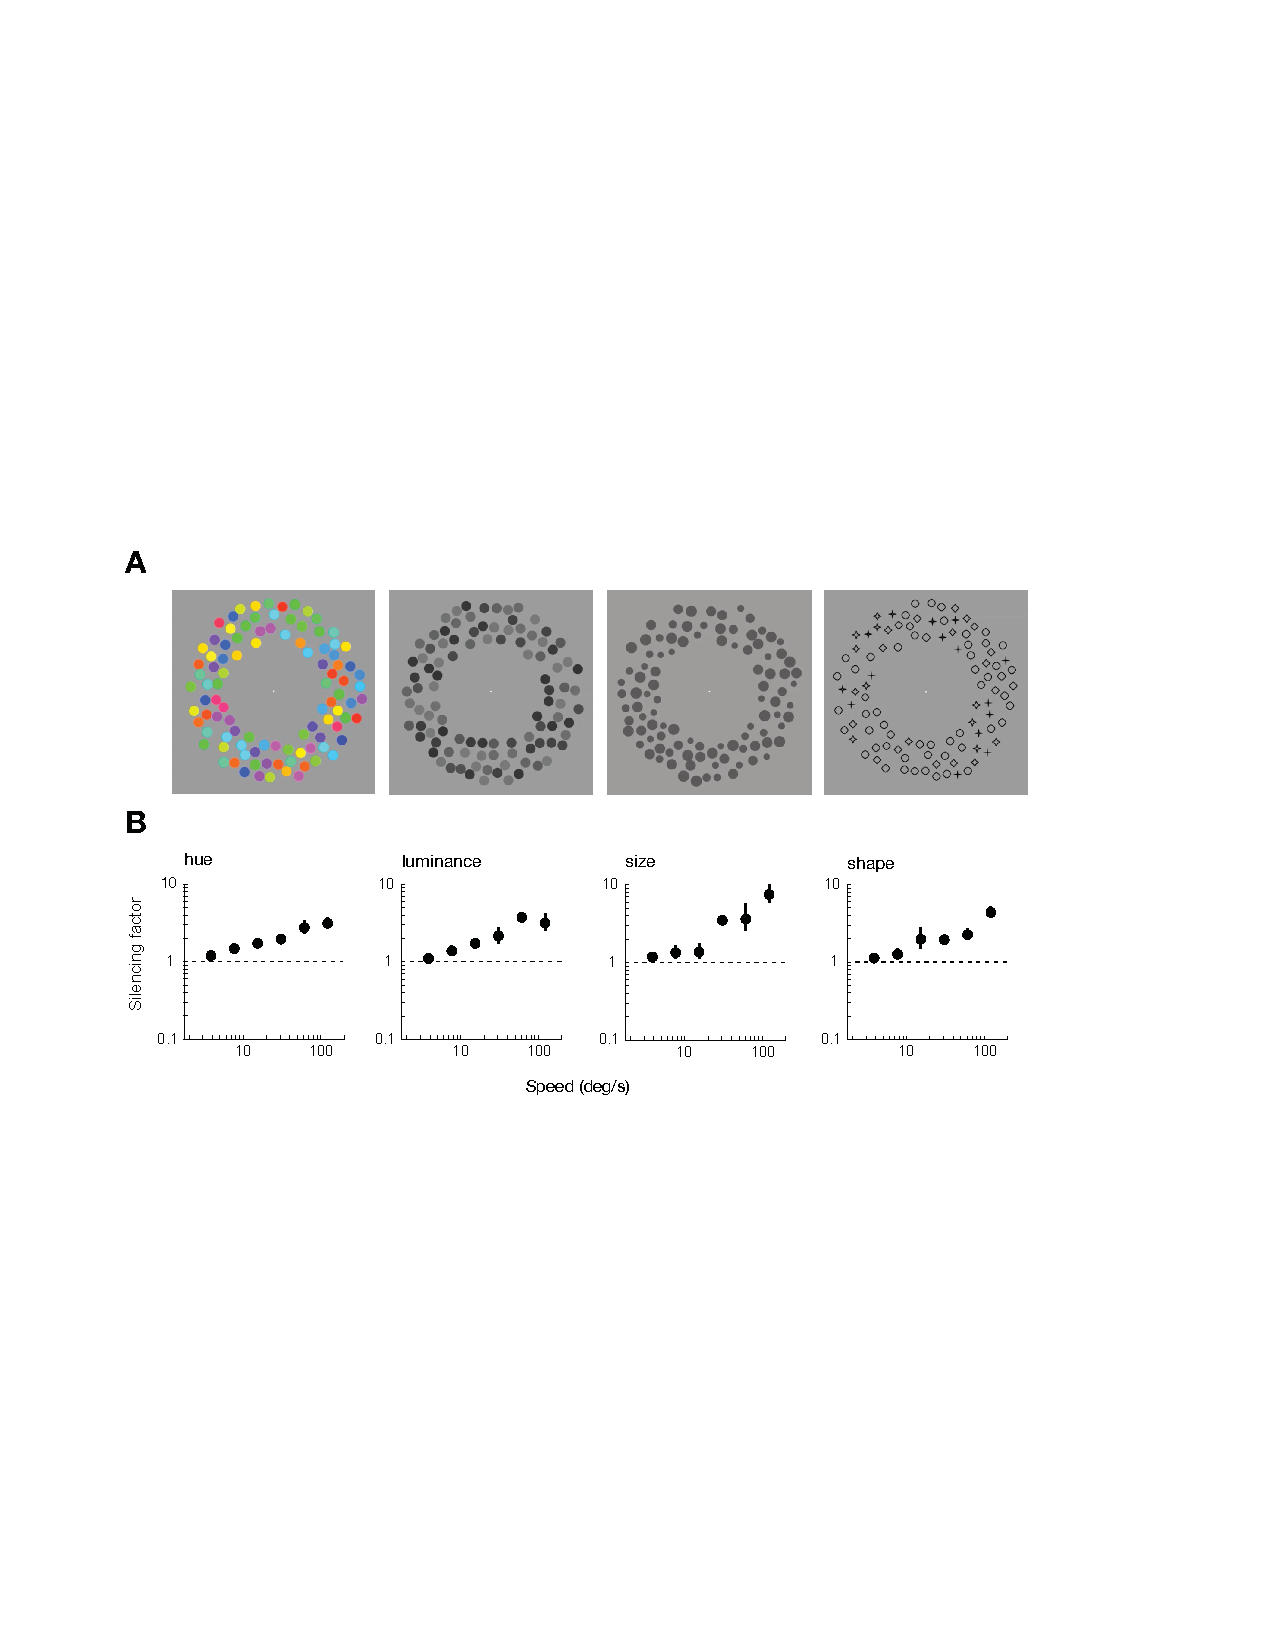
\includegraphics[width=\textwidth]{figures/fig1}
%\caption[Short figure name.]{This is a figure that %floats inline and here is its caption.
%\label{fig:myInlineFigure}}
%\end{figure}



%% Requires fltpage2 package
%%
% \begin{FPfigure}
% 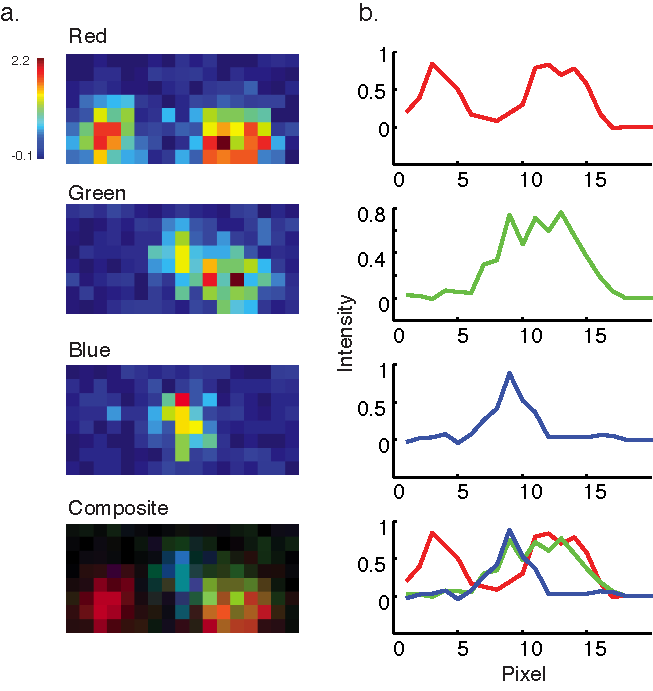
\includegraphics[width=\textwidth]{figures/fullpage}
% \caption[Short figure name.]{This is a full page figure using the FPfigure command. It takes up the whole page and the caption appears on the preceding page. Its useful for large figures. Harvard's rules about full page figures are tricky, but you don't have to worry about it because we took care of it for you. For example, the full figure is supposed to have a title in the same style as the caption but without the actual caption. The caption is supposed to appear alone on the preceding page with no other text. You do't have to worry about any of that. We have modified the fltpage package to make it work. This is a lengthy caption and it clearly would not fit on the same page as the figure. Note that you should only use the FPfigure command in instances where the figure really is too large. If the figure is small enough to fit by the caption than it does not produce the desired effect. Good luck with your thesis. I have to keep writing this to make the caption really long. LaTex is a lot of fun. You will enjoy working with it. Good luck on your post doctoral life! I am looking forward to mine. \label{fig:myFullPageFigure}}
% \end{FPfigure}
% \afterpage{\clearpage}
